	\newpage
\chapter{DESENVOLVIMENTO DO TRABALHO}

\par Objetivo desse capítulo é apresentar o desenvolvimento e a implantação do algoritmo para análise de dados.



\section{Coleta dos Dados}

\par Os dados depois de coletados e armazenados foram concedidos uma pequena amostra, mais ou menos oito meses de dados, no formato de xlsx (planilha \emph{Excel}) como pode ser observada na figura \ref{arquivo_de_dados}. Os dados têm  as informações de data hora da coleta a quantidade de litros consumidos por hora, e o total de litros acumulados. Com os dados em mãos foi inserido no \emph{jupyter notebook}, para realizar alguns experimentos, de \emph{data mining} com linguagem \emph{python} e suas bibliotecas.

\begin{figure}[ht]
	\caption{\textbf{Arquivo de Dados formato \emph{Excel}}}
	\centering
		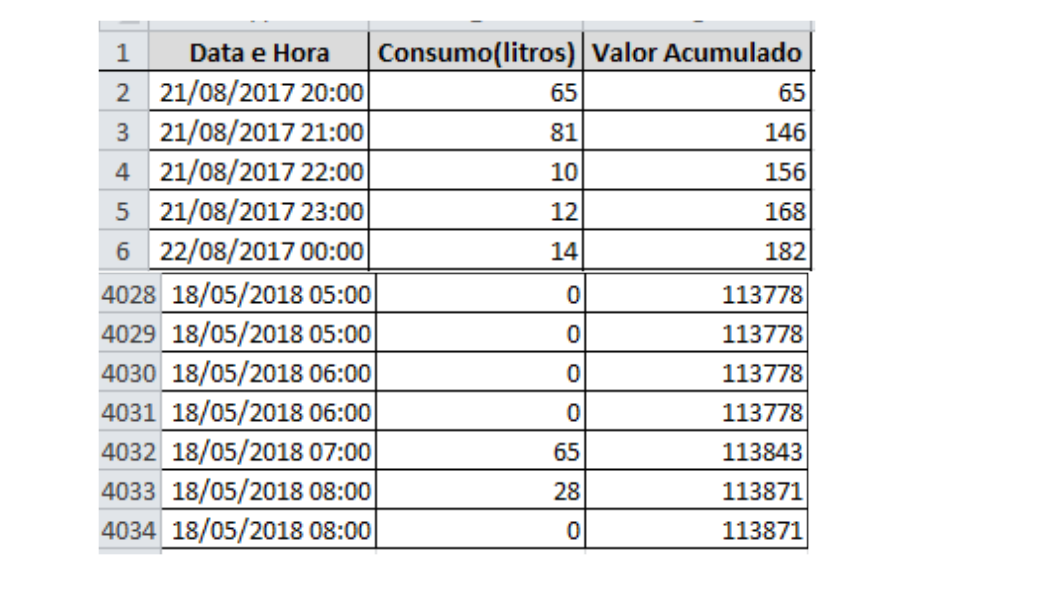
\includegraphics[width=\textwidth,height=\textheight, keepaspectratio]{figuras/planilhaexceldosdados3.png}
		\label{arquivo_de_dados}
	%\fonte{\cite{fayyad1996data}}
\end{figure}


\section{Desenvolvimento do algoritmo}

\begin{figure}[ht]
	\caption{\textbf{Importando as Bibliotecas}}
	\centering
		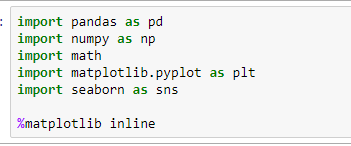
\includegraphics[scale=1, keepaspectratio]{figuras/importacaodasbibliotecas.PNG}
		\label{impor_b}
	%\fonte{\cite{fayyad1996data}}
\end{figure}

\par Como pode ser visualizado na figura \ref{impor_b}, o primeiro passo que deve ser feito é a importação das devidas bibliotecas para a análise dos dados. E é acrescentado um algoritmo na última linha o \emph{"\%matplotlib inline"} este por sua vez serve auxiliar a visualização na apresentação dos gráficos no \emph{jupyter notebook} sem a necessidade de utilizar a função especifica sendo está a \emph{“plt.show()”}.


\begin{figure}[ht]
	\caption{\textbf{Importação do arquivo}}
	\centering
		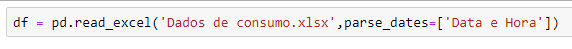
\includegraphics[scale=1, keepaspectratio]{figuras/importaroarquivo}
		\label{impor_arquivo}
	%\fonte{\cite{fayyad1996data}}
\end{figure}


\par Na figura \ref{impor_arquivo},  é   feita  a  importação do arquivo com os dados, atribui-se o arquivo com os dados a uma variável. Neste caso a variável denominada de "df", o  nome é dado comumente a uma variável, pois é a iniciais de um \emph{data frame}. Por sua vez um data frame é semelhante a uma matriz, mas as suas colunas tem nomes e podem conter dados de tipos diferentes. Um \emph{data frame} pode ser visto como uma tabela de uma base de dados, em que cada linha corresponde a uma registro da tabela. Cada coluna corresponde às propriedades, ou campos, a serem armazenadas para cada registro da tabela.  E   após  o  nome do arquivo  e  tipos do arquivo foi colocado uma função, \emph{"$parse_dates$"}, onde verifica a se as datas estão em um formato adequado para criação do \emph{data frame}.

\begin{figure}[ht]
	\caption{\textbf{Mostrando conteúdo do Data Frame}}
	\centering
		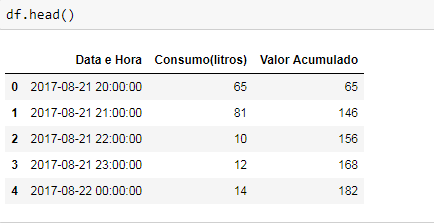
\includegraphics[scale=1, keepaspectratio]{figuras/mostraroconteudodoarquivo}
		\label{conteudo_df}
	%\fonte{\cite{fayyad1996data}}
\end{figure}

\par Ao executar este comando \emph{"df.head()"} podendo observar na figura \ref{conteudo_df}, é o conteúdo do \emph{data frame}. Verificando que o arquivo contém linhas e colunas, e que nas colunas compreende que contém data e hora em que o dado foi extraído, outra coluna a quantidade de litros de água consumidos e na outra coluna o valor acumulado de litros, a partir dá primeira extração dos dados. 

\begin{figure}[ht]
	\caption{\textbf{Separação da coluna Data e Hora}}
	\centering
		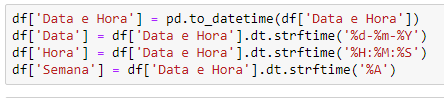
\includegraphics[scale=1, keepaspectratio]{figuras/organizararquivopordata}
		\label{separar_horaedata}
	%\fonte{\cite{fayyad1996data}}
\end{figure}

\par Após verificar o conteúdo do \emph{data frame}, é aplicado um algoritmo para desmembrar a coluna Data e Hora e criar outras colunas, como pode se observar na figura \ref{separar_horaedata}. Onde cada coluna recebeu os dados de acordo com as suas descrições, a coluna Data recebeu somente as datas, a coluna Hora recebeu somente as horas e foi criada uma coluna denominada de Semana, onde recebeu os dias da semana referenciando com a coluna Data.
\begin{figure}[ht]
	\caption{\textbf{Data Frame modificado}}
	\centering
		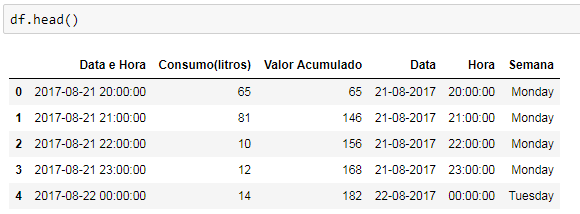
\includegraphics[scale=1, keepaspectratio]{figuras/mostrandoarquivoaposorganizacao}
		\label{arquivo_orga}
	%\fonte{\cite{fayyad1996data}}
\end{figure}

\par Na figura \ref{arquivo_orga} trata-se do \emph{data frame} que foi modificado para que as análises fossem realizadas com mais exatidão possível.

\begin{figure}[ht]
	\caption{\textbf{Funções \emph{Describe e mean}}}
	\centering
		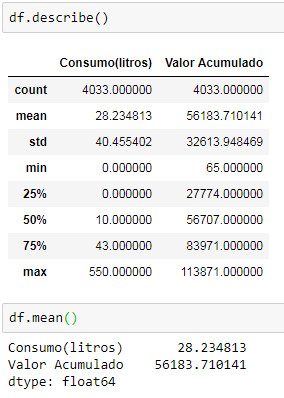
\includegraphics[scale=1, keepaspectratio]{figuras/describe-mean}
		\label{describe_mean}
	%\fonte{\cite{fayyad1996data}}
\end{figure}

\par Aplicando-se a função \emph{“df.describe”} no \emph{data frame}, como pode notar na figura \ref{describe_mean}, há o retorno de alguns dados estatísticos, onde o \emph{count} retorna a somatória de dados nesse caso total de 4033 dados para ambas as colunas, no caso do\emph{ mean} há o retorno das medias para todo o data frame, para a coluna consumo (litros) retorno de aproximadamente de 28 litros e na coluna valor acumulado o retorno de aproximadamente 56183 litros, onde se pode verificar o mesmo resultado a utilizar a função \emph{“df.mean()” } separadamente. No retorno do \emph{std}, que seria o desvio padrão, há o retorno na coluna de consumo (litros) de 40.455 e na coluna valor acumulado 32613.94. No caso do \emph{min} há o retorno de 0 litros na coluna de consumo (litros) e 65 na coluna valor acumulado, e no caso do \emph{“df.max ()”} há o retorno de 550 litros na coluna de consumo(litros) e 113871 na coluna de valor acumulado.

\begin{figure}[ht]
	\caption{\textbf{Algoritmo para plotagem dos dados}}
	\centering
		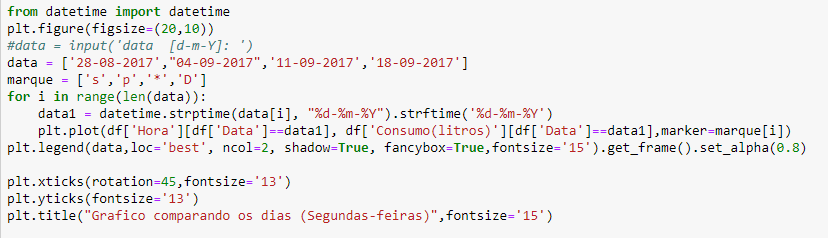
\includegraphics[width=\textwidth,height=\textheight , keepaspectratio]{figuras/codigograficoempython}
		\label{codigo_plotagem}
	%\fonte{\cite{fayyad1996data}}
\end{figure}

\par O Algoritmo na figura \ref{codigo_plotagem}, é utilizado para a plotagem dos dados, isso é o algoritmo serve para a visualização dos dados em forma de gráficos. Houve a importação da biblioteca \emph{datetime do python} para que se possa trabalhar com as datas. A função \emph{“plt.figure()”} é utilizada para formatar o tamanho da figura. Após é criada uma lista com algumas datas é atribuída a uma variável com nome de “data”, é feito o mesmo com a variável “marque”, mas recebendo uma lista com \emph{strings}, e com elas serão formados os marcadores do gráfico. Com um \emph{“for”} é feito uma iteração onde é passa por todos os elementos da lista “data”, e são adicionadas as datas separadas em uma variável “data1” onde é feita o tratamento para que possa ser realizada a plotagem de cada data na função \emph{“plt.plot()”}, se sendo assim também há iteração da lista dos marcadores onde cada data será plotada no gráfico tendo um marcador diferente, podendo assim fazer a comparação de cada data. E na função \emph{“plt.legend()”} é configurada a legenda do gráfico onde se podem ver os dados das datas diferente e realizando a comparação. Nas funções \emph{“plt.xticks”} e \emph{“plt.yticks()”} são configuradas os rótulos do gráfico tanto na horizontal como na vertical, ambas com o mesmo tamanho de fonte, mas o rotulo da horizontal tem uma pequena diferença a configuração da rotação dos rótulos para 45º para facilitar a visualização. E por fim \emph{“plt.title()”} onde é configurado o título do gráfico com a fonte tamanho 15. 

\begin{figure}[ht]
	\caption{\textbf{Função para calculo das médias diárias}}
	\centering
		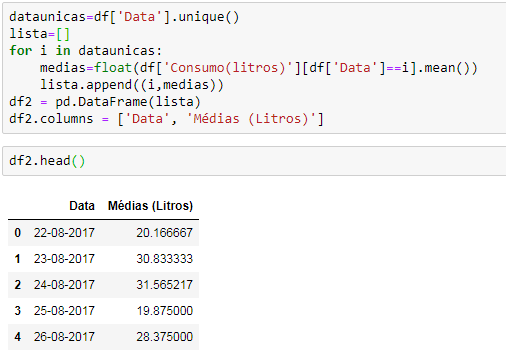
\includegraphics[scale=1, keepaspectratio]{figuras/codigoparacalculodemediasdiarias}
		\label{codigo_medias_diarias}
	%\fonte{\cite{fayyad1996data}}
\end{figure}

\par Com esta função que está na figura \ref{codigo_medias_diarias}, foi obtida às médias diárias. Primeiramente foi denominada uma variável “dataunicas” onde recebeu as datas dos dados, e utilizando se um \emph{for} para se fazer uma iteração para o cálculo da média, e foi armazenado em uma lista em forma de tuplas. Cada tupla recebeu a data e a média correspondente a aquela data. Após ter a lista completa foi criada uma variável, denominada “df2”, onde recebeu um novo \emph{dataframe}, e com o comando \emph{“columns”} nomeiando se as colunas desse novo dataframe, onde foi exibido na figura \ref{codigo_medias_diarias} logo abaixo do algoritmo.


\section{Aplicando a formula da Distância Euclidiana em Python}

\begin{figure}[ht]
	\caption{\textbf{Exemplo de Distância Euclidiana em \emph{Python}}}
	\centering
		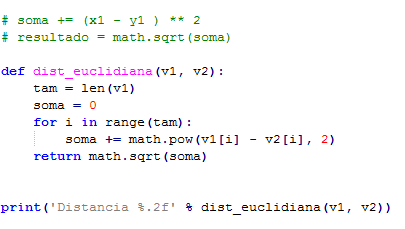
\includegraphics[scale=1, keepaspectratio]{figuras/codigodistanciaeuclidianaempython}
		\label{dist_eu_py}
	%\fonte{\cite{fayyad1996data}}
\end{figure}

\begin{figure}[h]
	\caption{\textbf{Exemplo de Distância Euclidiana em \emph{Python} com biblioteca \emph{Numpy}}}
	\centering
		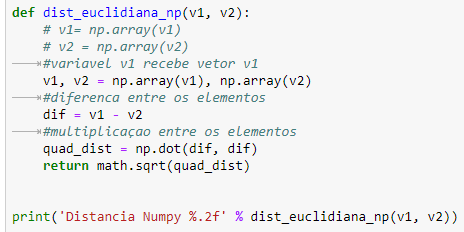
\includegraphics[scale=1, keepaspectratio]{figuras/codigodistanciaeuclidianaempythonnumpy}
		\label{dist_eu_pynumpy}
	%\fonte{\cite{fayyad1996data}}
\end{figure}

\par Como é visto  nas figuras \ref{dist_eu_py} e na figura \ref{dist_eu_pynumpy},aplicações de funções da Distância Euclidiana em \emph{Python}, sendo que na figura \ref{dist_eu_pynumpy} foi aplicada a formula da Distância Euclidiana com auxilio da biblioteca \emph{Numpy}, notando se que as variáveis v1 e v2 são vetores que recebem listas com uma amostragem de dados, nesse caso uma série de números variados, após isso é feito a diferença nas variáveis que na verdade são matrizes, e depois é realizada a multiplicação entre as matrizes e depois é retornada a raiz quadrada das matrizes, e é verificado o cálculo obtendo o resultado que tende a ser o mais próximo de zero, para poder demostrar um agrupamento de padrões nos dados.


